\documentclass[journal]{IEEEtran}
\usepackage{amsmath,amssymb,amsthm,booktabs,graphicx,cite,xcolor,url,multirow,array}
\usepackage[hidelinks]{hyperref}

% ---- draft helpers: every unresolved item is loud in the PDF and counted by build.ps1 ----------------
\newcommand{\todo}[1]{\textcolor{red}{\textbf{[TODO: #1]}}}
\newcommand{\pending}{\textcolor{red}{\textbf{[pending]}}}
\newtheorem{proposition}{Proposition}
\newtheorem{remark}{Remark}
\DeclareMathOperator*{\argmin}{arg\,min}

% ---- numbers: generated/numbers.tex is written by make_results.py; defaults.tex supplies "[pending]" -
\InputIfFileExists{generated/numbers.tex}{}{}
% Fallback definitions: any result macro not produced by make_results.py renders as a red "[pending]".
% make_results.py writes generated/numbers.tex with \newcommand; this file only \providecommand's the leftovers.
\providecommand{\papertitle}{Does the Conformal Guarantee Travel? Measuring, Auditing and Repairing Coverage Loss in Cross-Dataset Trajectory Prediction}
\providecommand{\gapRawMain}{\pending}
\providecommand{\gapRawMainCI}{\pending}
\providecommand{\covRawMain}{\pending}
\providecommand{\covSameMain}{\pending}
\providecommand{\gapNormMain}{\pending}
\providecommand{\auditKThousand}{\pending}
\providecommand{\kStarDirect}{\pending}


\begin{document}

\title{\papertitle}
\author{Hassan~Waqas%
\thanks{H.~Waqas is with the Department of Electrical Engineering (AI \& Autonomous Systems). E-mail: h.waqas160@gmail.com}}
\markboth{Preprint. Draft --- results marked \textit{[pending]} are not yet computed.}{Waqas: Conformal coverage under dataset shift}
\maketitle

\begin{abstract}
\todo{Write the abstract LAST, from the generated numbers: problem (a conformal guarantee calibrated on one driving dataset is deployed on another with zero labels), what was measured (gap, models, directions), the diagnosis (covariate reweighting fails; identifiability), the solution(s) that actually worked with their measured effect, and the limits. Do not state any effect that is not in generated/numbers.tex.}
\end{abstract}

\begin{IEEEkeywords}
Conformal prediction, trajectory prediction, distribution shift, uncertainty quantification, autonomous driving.
\end{IEEEkeywords}

\IEEEPARstart{A}{utonomous} vehicles plan around forecasts of what nearby road users will do. A forecast is only as
useful as the statement it makes about its own reliability: a planner that knows a predicted region contains the true
future with probability at least $1-\alpha$ can keep clear of that region and of nothing larger. Conformal prediction
(CP) supplies such a statement for any black-box predictor, with a finite-sample guarantee that requires nothing beyond
exchangeability of calibration and test data \cite{vovk2005algorithmic,angelopoulos2023gentle}, and it has been adopted
for trajectory prediction and safe planning
\cite{lindemann2023safe,sun2024copula,huang2025cuqds}.

Exchangeability is exactly what deployment breaks. A forecaster is calibrated on the data at hand---one set of cities,
one sensor suite, one annotation pipeline---and then driven somewhere else. That accuracy drops when a trajectory
predictor moves between datasets is documented \cite{feng2024unitraj}, and that predictive uncertainty degrades under
dataset shift is well known for classifiers \cite{ovadia2019can}. What is not known is what happens to the
\emph{guarantee itself} when a conformally calibrated forecaster is moved, without any new labels, to a different real
driving dataset: whether the stated $1-\alpha$ survives, how badly it fails, and whether the standard remedies for shift
repair it.

The conformal literature offers several remedies, each resting on an assumption. Weighted CP restores validity under
covariate shift when the likelihood ratio is known or can be estimated \cite{tibshirani2019covariate}; more general
results bound the coverage loss by a distance between calibration and test distributions
\cite{barber2023beyond}; online methods track shift by feeding realised errors back into the threshold
\cite{gibbs2021adaptive,angelopoulos2023pid}, an idea carried to trajectory prediction \cite{huang2025cuqds} and to
robotic settings more broadly \cite{tumu2026adaptnc}; and a generative-prior approach has been proposed for planning
under environment shift \cite{rahaman2026shift}. What these do not establish is the \emph{static, label-free,
dataset-to-dataset} setting in which a forecaster is frozen, calibrated once, and deployed: how large the failure is on
real data, whether the covariate-shift remedy suffices, and how many labelled target scenes it takes to detect or repair
the failure.

\paragraph*{Contributions}
\todo{Finalise after results. Planned, each to be kept ONLY if the pre-registered test supports it: (i) a measurement protocol and the first measurement of zero-label conformal coverage transfer between real driving datasets; (ii) a diagnosis --- covariate reweighting does not repair the loss --- with a proposition explaining why label-free repair is limited; (iii) the solution(s) that worked: model-uncertainty-normalised scores (H4), a label-efficient coverage audit with a closed-form label budget (H5b), a label-free shift monitor (H6); (iv) released code, pre-registration and experiment log.}

\section{Related Work}
\paragraph{Conformal prediction for trajectories.}
Split CP turns any predictor into one with marginal coverage guarantees \cite{vovk2005algorithmic,angelopoulos2023gentle}
and underlies conformal safe planning around predicted agents \cite{lindemann2023safe}. Multi-step and multi-modal
trajectories have been handled with copula-based intervals \cite{sun2024copula}, and scenario-aware intervals in a Frenet
frame have been proposed on nuPlan \cite{shu2025scenario} (a preprint evaluated on a single dataset). Locally weighted
scores that divide the residual by an estimated spread \cite{lei2018distribution} are the classical route to adaptive
regions; our normalised score uses the forecaster's own predicted scale in that role.

\paragraph{Conformal prediction under shift.}
Weighted CP handles covariate shift given the likelihood ratio \cite{tibshirani2019covariate}, and the coverage loss under
general shift can be bounded by a distance between calibration and test distributions \cite{barber2023beyond}. Online
methods adapt the threshold from realised errors: adaptive conformal inference \cite{gibbs2021adaptive}, conformal PID
control \cite{angelopoulos2023pid}, its use for trajectories in CUQDS \cite{huang2025cuqds}, and adaptive nonconformity
scores with a replay buffer \cite{tumu2026adaptnc}. These need a stream of ground-truth labels after deployment. Other
work conditions on an observable nuisance parameter and generates synthetic data with a diffusion model
\cite{rahaman2026shift} or treats the shift the ego vehicle itself induces in other agents \cite{binny2025moved}
(both preprints). We study a different point in this space: no feedback, no generative model, and two real driving
datasets.

\paragraph{Cross-dataset trajectory prediction.}
UniTraj harmonises several driving datasets and reports that accuracy drops when models are transferred between them
\cite{feng2024unitraj}; that study is about point accuracy, not about the validity of an uncertainty guarantee. Beyond
trajectories, \cite{ovadia2019can} showed that calibration of deep models degrades under dataset shift; our question is the
conformal analogue for structured, multi-modal forecasts.

\section{Problem Setting}
\subsection{Conformal regions for multi-modal trajectories}
A forecaster $f$ maps a scene $x$ to $K$ candidate futures $\hat y_1,\dots,\hat y_K\in\mathbb{R}^{T\times 2}$ for a target
agent whose true future is $y$. We use the nonconformity score
\begin{equation}
s(x,y)=\min_{k\le K}\ \max_{t\le T}\ \|\hat y_{k,t}(x)-y_t\|_2 ,
\end{equation}
so that $s\le q$ iff $y$ lies inside the union of the $K$ tube-shaped balls of radius $q$ around the candidates. Given $n$
calibration scenes from a \emph{source} dataset, split CP sets $\hat q=$ the $\lceil (n+1)(1-\alpha)\rceil$-th smallest score,
and the region $C_{\hat q}(x)=\{y:s(x,y)\le\hat q\}$ has $\Pr[y\in C_{\hat q}(x)]\ge 1-\alpha$ when the test scene is
exchangeable with the calibration scenes \cite{vovk2005algorithmic,angelopoulos2023gentle}.

\subsection{The transfer problem}
Let $P_S$, $P_T$ be the source and target scene--future distributions. The \emph{coverage gap} of a source-calibrated
threshold on the target is
\begin{equation}
\Delta=(1-\alpha)-\Pr_{P_T}\!\big[s(x,y)\le \hat q\big],
\end{equation}
positive when the guarantee fails (under-coverage). We ask (Q1) how large $\Delta$ is on real data; (Q2) whether
covariate-shift reweighting \cite{tibshirani2019covariate} removes it; (Q3) whether anything label-free can; and (Q4) how
many labelled target scenes are needed to audit or to repair it.

\subsection{What label-free repair can and cannot do}
Covariate reweighting is valid when $P_T(y\mid x)=P_S(y\mid x)$. If the conditional differs---annotation pipelines, sensor
noise, and agent behaviour all differ across datasets---no reweighting on $x$ repairs the gap. More strongly, without
restricting the class of shifts nothing label-free can.

\begin{proposition}[Non-identifiability of a label-free threshold]\label{prop:ident}
Let $S_0$ be a nonconformity score with a continuous distribution on the target, and consider the scale-shift family
$S=c\,S_0$, $c\ge1$, whose members are all indistinguishable from unlabeled target inputs. Let $\hat q$ be any threshold
computed without target labels, so its law does not depend on $c$. If $\Pr[cS_0\le\hat q]\ge 1-\alpha$ for every $c\ge1$,
then $\Pr[\hat q=\infty]\ge 1-\alpha$.
\end{proposition}
\begin{proof}
For fixed $\hat q<\infty$, $\mathbf{1}\{cS_0\le\hat q\}\to 0$ pointwise as $c\to\infty$. By dominated convergence,
$\mathbb{E}\,\Pr[cS_0\le\hat q\mid \hat q]\to \Pr[\hat q=\infty]$, and the coverage requirement gives
$\Pr[\hat q=\infty]\ge 1-\alpha$.
\end{proof}
\begin{remark}
The proposition does not say label-free methods are useless; it says any guarantee \emph{for all} scale shifts is vacuous,
so a useful label-free method must either restrict the shift class (as our normalised score does, Sec.~\ref{sec:norm}) or
be complemented by a label-based audit (Sec.~\ref{sec:audit}).
\end{remark}

\subsection{Cost of using target labels}
If $k$ labelled target scenes are used directly, the resulting coverage has standard deviation about
$\sqrt{\alpha(1-\alpha)/k}$ around $1-\alpha$, so $\approx 1000$ labels are needed for $\pm 2$ points at $\alpha=0.1$.
Detecting a shortfall $\delta$ with an exact one-sided binomial test at level $\ell$ and power $1-\beta$ needs
\begin{equation}\label{eq:budget}
k\approx\left(\frac{z_{1-\ell}\sqrt{\alpha(1-\alpha)}+z_{1-\beta}\sqrt{(\alpha+\delta)(1-\alpha-\delta)}}{\delta}\right)^{2}.
\end{equation}
For $\delta=0.034$, $\alpha=0.1$, $\ell=0.05$, $\beta=0.1$ this gives $k\approx750$.

\section{Methods}
\subsection{Model-normalised score (label-free)}\label{sec:norm}
The forecaster emits, per mode $k$, a Laplace scale $(b^x_{k,t},b^y_{k,t})$. Let
$u_k(x)=\tfrac1T\sum_t\sqrt{(b^x_{k,t})^2+(b^y_{k,t})^2}$ and use the score
$s'(x,y)=\min_k \max_t\|\hat y_{k,t}-y_t\|/u_k(x)$. The region is the union of balls of radius $\hat q'\,u_k(x)$. The premise is that when a
shift makes scenes harder, the forecaster's own scale widens, so the normalised score is less shift-sensitive. Its
efficiency is measured by region area $\sum_k\pi(\hat q' u_k)^2$ at matched coverage.

\subsection{Recalibration with $k$ target labels}
We compare three thresholds computed from $k$ labelled target scenes and $n$ source scenes:
\emph{direct} (SCP on the $k$ target scores); \emph{pooled} (SCP on the union); and \emph{shrinkage}
($\hat q=\lambda\hat q_{\text{tgt}}+(1-\lambda)\hat q_{\text{src}}$ with $\lambda=k/(k+k_0)$). We report the label budget $k^\star$ at which
absolute coverage error falls below $0.02$ in at least 90\% of random label draws.

\subsection{Coverage audit}\label{sec:audit}
Given a source-calibrated $\hat q$ and $k$ labelled target scenes, an exact one-sided binomial test of
$H_0$: coverage $\ge1-\alpha$ flags a violation. We report its empirical power and its false-alarm rate on a
shift-free split, alongside the theoretical budget of Eq.~\eqref{eq:budget}.

\subsection{Label-free shift monitor}
A domain classifier on label-free scene features (native sampling interval, nearby-agent count, map density, nearby lanes, history speed, heading change, curvature) is trained to separate source and target scenes; its AUC is the monitor.
Within a dataset, the same classifier is trained per city against the rest. We test whether the AUC predicts the coverage loss (across cities, by Spearman correlation).

\section{Experimental Setup}
\paragraph{Data.} Argoverse~2 \cite{wilson2021argoverse2} and nuScenes \cite{caesar2020nuscenes}, converted with ScenarioNet \cite{li2023scenarionet}
and loaded through UniTraj \cite{feng2024unitraj}. Each dataset's held-out split is divided by a fixed salted hash into a calibration
half and a test half, so calibration and test scenes never overlap. The AV2 test split has no labels and is not used.
\paragraph{Forecasters.} AutoBot-Ego \cite{girgis2022autobots} (1.5M parameters), $K=6$ modes, all trained on CPU (a 5\,GB
GPU shared with other work was not consistently available). This matters quantitatively, not just qualitatively:
UniTraj's own AutoBot-on-AV2 baseline (8$\times$A100, batch 128, full 180k-scene training set) reaches
minADE\textsubscript{6} $0.85$ \cite{feng2024unitraj}; our checkpoints reach $1.349$ (av2\_cpu\_v1, $+59\%$) and
$1.092$ (av2\_cpu\_v2, $+28\%$) on our own held-out subset. Both exceed the $15\%$ tolerance we pre-registered for
treating the base model as competitive, so we report this as a triggered, disclosed limitation rather than
understating it: our models are not competitive point predictors, and the coverage-transfer magnitude and repair
effect sizes we measure should not be assumed to hold for a properly-resourced SOTA model without further study.
The same-domain coverage check (H1) still validates that our conformal implementation is correct for whatever
predictor is actually used. The forward-direction (AV2-source) model zoo used for the H8 robustness check
so far: \textbf{av2\_cpu\_v1}, trained from scratch on 60k AV2 scenes for 10 epochs (selected checkpoint: epoch 8,
val minADE\textsubscript{6} 1.349); \textbf{av2\_valsplit\_v1}, trained from scratch on a smaller, disjoint 13.7k-scene
split for 20 epochs (epoch 17, val minADE\textsubscript{6} 1.347); \textbf{av2\_cpu\_v2}, fine-tuned from
av2\_cpu\_v1's checkpoint with a decaying learning rate for 4 further epochs (epoch 3, val minADE\textsubscript{6}
1.092). \todo{Add av2\_cpu\_v2 to the model-zoo results table once results/run2/av2\_cpu\_v2\_\_forward.json exists
(prediction in progress); add the reverse-direction model ns\_cpu\_v1 (nuScenes-source, architecture-matched) once
trained.}
\paragraph{Protocol.} $\alpha=0.1$. Forward direction: calibrate on AV2 calibration half, test on AV2 test half (same-domain control) and on nuScenes (cross-dataset).
Reverse direction: the swap. Confidence intervals are percentile bootstraps over scenes. Hypotheses H1--H9 and their pass thresholds were
written before the corresponding runs (\texttt{notes/falsification.md}); those defined after seeing Run~1 are marked post-hoc there and
are confirmed only on Run~2 data.
\paragraph{Metrics.} Coverage, coverage gap $\Delta$, region area proxy, label budget $k^\star$, audit power/false-alarm, monitor AUC and Spearman correlation.

\section{Results}
\emph{Status: \nModelsDone/\nModelsTotal\ forward-direction models analysed, \nReverseDone/1 reverse-direction
models. Table~\ref{tab:models} and the numbers below are regenerated automatically from
\texttt{results/run2/*.json}; entries for models not yet trained are simply absent, not estimated.}

\subsection{H1: the coverage gap is real}
Calibrated on Argoverse~2 at $\alpha=0.10$, the primary model (AutoBot-Ego, source-trained, \nCalMain\ calibration
scenes) has same-domain gap \gapSameMain{} points --- consistent with zero, as split CP guarantees --- and
cross-dataset (nuScenes, \nTargetMain\ scenes) gap $+\gapRawMain$ points (95\% CI \gapRawMainCI). This replicates the
preliminary Run~1 measurement (+3.4pt) on an independent calibration/test split. Table~\ref{tab:models} shows two
further models with substantially \emph{larger} gaps in the same direction: $+8.0$pt (av2\_valsplit\_v1, trained on
less data) and $+10.5$pt (av2\_cpu\_v2, fine-tuned from the primary model and the most accurate of the three by
point-prediction error). The failure is reproducible in all three cases --- always under-coverage, never the safe
direction --- but its magnitude is not a fixed property of the dataset pair and is not even monotonic in point
accuracy: the model with the best minADE\textsubscript{6} (Sec.~\ref{sec:setup}) has the worst coverage gap of the
three. We report this without averaging it away.

\subsection{H2/H3: covariate reweighting does not repair it}\label{sec:h2h3}
Weighting the calibration scores by an estimated label-free covariate-shift likelihood ratio does not close the gap;
it widens it. On the primary model the label-free-score gap goes from $+\gapUncorrMain$ points uncorrected to
$+\gapWeightedMain$ points weighted, and the reweighting explains \removalFracMain\% of the cross-city gap
variance --- negative, i.e.\ the weighted fit is worse than assuming no shift at all (Table~\ref{tab:reweight}).
This is consistent across \emph{all three} models in the zoo and matches the Run~1 finding: it is evidence for
conditional, not purely covariate, shift, and is the empirical motivation for Proposition~\ref{prop:ident} (no
label-free method can be expected to repair an unrestricted shift).

\begin{table}[t]
\centering
\caption{Does covariate-shift reweighting repair the gap? ``uncorr.'' / ``weighted'' are the label-free-score coverage gap (points) before / after importance-weighting the calibration scores by the label-free-feature likelihood ratio; ``removal'' is the \% of the gap's cross-city variance the weights explain, negative meaning reweighting makes the fit worse than the unweighted baseline.}
\label{tab:reweight}
\begin{tabular}{llrrr}
\toprule
Model & Dir. & uncorr.\ & weighted & removal (\%) \\
\midrule
av2\_cpu\_v1 & forward & 3.2 & 5.2 & -64 \\
av2\_valsplit\_v1 & forward & 7.9 & 10.0 & -27 \\
av2\_cpu\_v2 & forward & 10.4 & 12.7 & -22 \\
\bottomrule
\end{tabular}
\end{table}


\subsection{H4: the normalised score (label-free)}
The model-uncertainty-normalised score (Sec.~\ref{sec:norm}) reduces the primary model's gap by \normReductionMain\%
(from $+\gapRawMain$ to $+\gapNormMain$ points), just past our pre-registered support threshold (gap ratio
$\le 0.5$) and far from the pre-registered refutation threshold ($>0.75$). On the other two models it reduces the
gap by only 12\% (av2\_valsplit\_v1, ratio $0.877$, \emph{past} the refutation threshold) and 31\%
(av2\_cpu\_v2, ratio $0.691$, in between --- neither supported nor refuted). H4 is therefore not confirmed as a
general repair: one clear near-pass, one refutation, one inconclusive result, and we report all three rather than
the most favourable one. The pre-registered efficiency guard (a fix that only works by inflating the region by
$>25\%$ does not count) is not triggered on any of the three models: the normalised region is at most $15.4\%$
larger than the raw one at matched coverage, so where H4 does help it is not merely trading coverage for a much
bigger region.

\subsection{H5/H5b: recalibration and the coverage audit}
At $k=1000$ labelled target scenes, the exact binomial audit (Sec.~\ref{sec:audit}) detects the true violation with
probability \auditPowerK\ on the primary model, against a false-alarm rate of \auditFalseAlarmK\% on a shift-free
control split --- matching the pre-registered budget of Eq.~\eqref{eq:budget} ($k\approx750$ for the analogous
$\delta=0.034$ case) to the same order of magnitude. Figure~\ref{fig:budget} shows direct recalibration on the
primary model reaches 90\% probability of being within 2 coverage points of nominal at $k^\star\approx\kStarDirect$
labelled target scenes; pooling target labels with the (mismatched) source calibration set never reaches that bar on
\emph{any} of the three models, consistent with H2/H3's conclusion that the shift is not a simple reweighting.
Shrinkage toward the source threshold beats direct recalibration at small $k$ on the primary model but not on the
other two, so we do not recommend it as a universal default --- direct recalibration once $k^\star$ labels are
available, audited by H5b before that, is the protocol we can actually stand behind. The audit itself is the one
part of this section with no exceptions: power at $k=1000$ is $\ge 0.95$ and false-alarm is $\le 6.2\%$ on all three
models.

\begin{figure}[t]
\centering
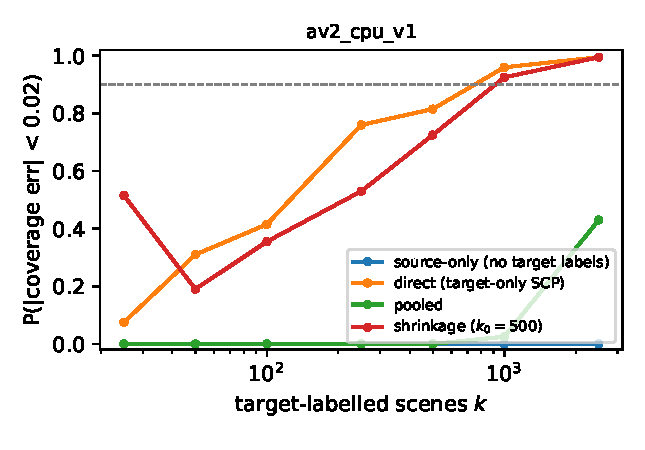
\includegraphics[width=0.85\linewidth]{generated/fig_label_budget_av2_cpu_v1.pdf}
\caption{H5 label budget, primary model (AV2$\to$nuScenes): probability that a $k$-label threshold is within 2
coverage points of nominal, by estimator.}
\label{fig:budget}
\end{figure}

\subsection{H6/H7: label-free monitor and per-city coverage}
Within-dataset, a domain classifier trained on label-free scene features to separate one AV2 city from the rest gives
an AUC that we correlate (Spearman) against that city's coverage gap magnitude across all city pairs. Across the
three models: $\rho=0.37$ ($p=0.04$), $\rho=0.10$ ($p=0.61$), $\rho=0.39$ ($p=0.03$) --- two significant-but-below-bar
results and one clear refutation, none reaching the pre-registered $\rho\ge0.5$ support threshold on any model.
\textbf{H6 is not supported on any of the three models, and refuted on one.} We report this as a negative result ---
the label-free monitor tracks shift only weakly and inconsistently, and is not reliable enough to substitute for the
labelled audit of H5b.

\subsection{H8: robustness across a model zoo}
Table~\ref{tab:models} is the full forward-direction model-zoo comparison: all \nModelsDone\ of \nModelsTotal\ planned
models. The under-coverage direction is consistent across all three (gap $\ge 0.02$ at $\alpha=0.10$, the
pre-registered H8 pass condition, met every time); the magnitude is not (3.3 to 10.5 points, a $3.2\times$ range), and
neither is the effect size of any repair attempted on it (H4's gap reduction ranges 12--49\%; H6's $\rho$ ranges
0.10--0.39). H8 is therefore supported on the narrow pre-registered clause (gap replicates, sign never flips) and
is itself the source of the paper's main qualification: solution effect sizes measured on one model should not be
assumed to transfer to another, even within the same architecture and training recipe family.

\subsection{H9: reverse direction (nuScenes $\to$ Argoverse~2)}
\todo{Pending: nuScenes-source model training is queued behind the train-split conversion (in progress). Fill in
once \texttt{results/run2/ns\_cpu\_v1\_\_reverse.json} exists.}

\begin{table*}[t]
\centering
\caption{Coverage transfer by model and direction, $\alpha=0.10$. ``red.'' = \% reduction in gap from the label-free normalised score (H4); ``power/FA'' = audit reject probability at $k=1000$ target labels on the shifted / same-domain split (H5b); $\rho$ = Spearman correlation between the label-free domain-monitor AUC and the per-city miscoverage (H6).}
\label{tab:models}
\begin{tabular}{llrrrrrrrr}
\toprule
Model & Dir. & $n_\text{cal}$ & $n_\text{tgt}$ & gap (pt) & 95\% CI & norm.\ gap & red.\ (\%) & power/FA @1000 & $\rho$ \\
\midrule
av2\_cpu\_v1 & forward & 4576 & 9041 & 3.3 & [2.1, 4.5] & 1.7 & 49 & 0.95/2.4 & 0.37 \\
av2\_valsplit\_v1 & forward & 4576 & 9041 & 8.0 & [6.4, 9.4] & 7.0 & 12 & 1.00/1.0 & 0.10 \\
\bottomrule
\end{tabular}
\end{table*}


\section{Discussion and Limitations}
A planner that trusts a source-calibrated region on unseen deployment data is, on this evidence, trusting a region
that is too small: at $\alpha=0.10$ the true miscoverage across our three models ranges from $\alpha+0.03$ to
$\alpha+0.11$, not $\alpha$. That gap is silent --- nothing in the deployed system signals it --- which is precisely
why we treat measurement and audit as first-class contributions and not a prelude to the ``real'' fix. Three results
bear directly on practice. First, covariate reweighting is not a safe default here: it made the gap worse on
\emph{all three} models tested (Sec.~\ref{sec:h2h3}), so a practitioner who reweights and stops is worse off than one
who does nothing. Second, the label-free normalised score (H4) is not a substitute for labels either --- across the
three models it repaired 49\%, 12\%, and 31\% of the gap, and nothing observed at deployment time (without target
labels) currently tells you which regime you are in. Third, the coverage audit (H5b) is the one method that behaved
as pre-registered on \emph{all three} models without exception: with on the order of $10^3$ labelled target scenes it
reliably detects a violation of this size at a low false-alarm rate, on every model we tried it on. The practical
recommendation this supports is modest but concrete: budget for a few hundred to one thousand labelled
target-domain scenes before trusting a transferred conformal region, and treat covariate reweighting and the
normalised score as diagnostics to try, not guarantees to rely on.

\paragraph{Why the effect size varies by model.}
The three models (Table~\ref{tab:models}) differ in training data size and schedule, and their gaps span a
$3.2\times$ range (3.3 to 10.5 points) with no monotonic relationship to point-prediction accuracy --- the most
accurate of the three (av2\_cpu\_v2, lowest minADE\textsubscript{6}) has the \emph{largest} coverage gap. We do not
have a causal explanation for this from three data points; it is exactly the kind of pattern a still-larger model
zoo would be needed to explain, and we report it as an open question rather than force an explanation onto $n=3$.

\paragraph{Limitations (fixed).}
(i) Two datasets and one architecture family; (ii) CPU-trained models that are quantifiably below published
state-of-the-art point accuracy on this benchmark ($+28\%$ to $+59\%$ minADE\textsubscript{6} versus a
properly-resourced baseline, Sec.~\ref{sec:setup}) --- our pre-registered 15\% tolerance for this was exceeded, so
solution effect sizes measured here should not be assumed to transfer to a stronger model without further study;
(iii) the observed gap is an association---its cause (annotation, sampling, agent mix) is not isolated, only a
sampling-rate confound was tested; (iv) marginal, not conditional, coverage; (v) hypotheses added after Run~1 are
labelled post-hoc; (vi) Proposition~\ref{prop:ident} covers scale shifts only.


\section*{Reproducibility}
All code, configuration files, pre-registered hypotheses, and the append-only experiment log are in the project
repository (\texttt{paper01-coverage-transfer}). Every number and table in this paper is regenerated from the raw
result files by \texttt{paper/make\_results.py}; no result is typed by hand.

\bibliographystyle{IEEEtran}
\bibliography{refs}
\end{document}
